\section{Design of a Service Mesh Benchmarking Instrument}
\label{sec:system:design}

In this section, we present the design for \textit{MeshBench}, a benchmarking instrument for \gls{sm} systems. In \cref{fig:benchmark-design} we depict an overview of the benchmark and its components where each component is annotated. The remainder of this section will introduce these components individually, and address their respective roles in the benchmark.



\begin{figure}[!t]
    \centering
    
     
    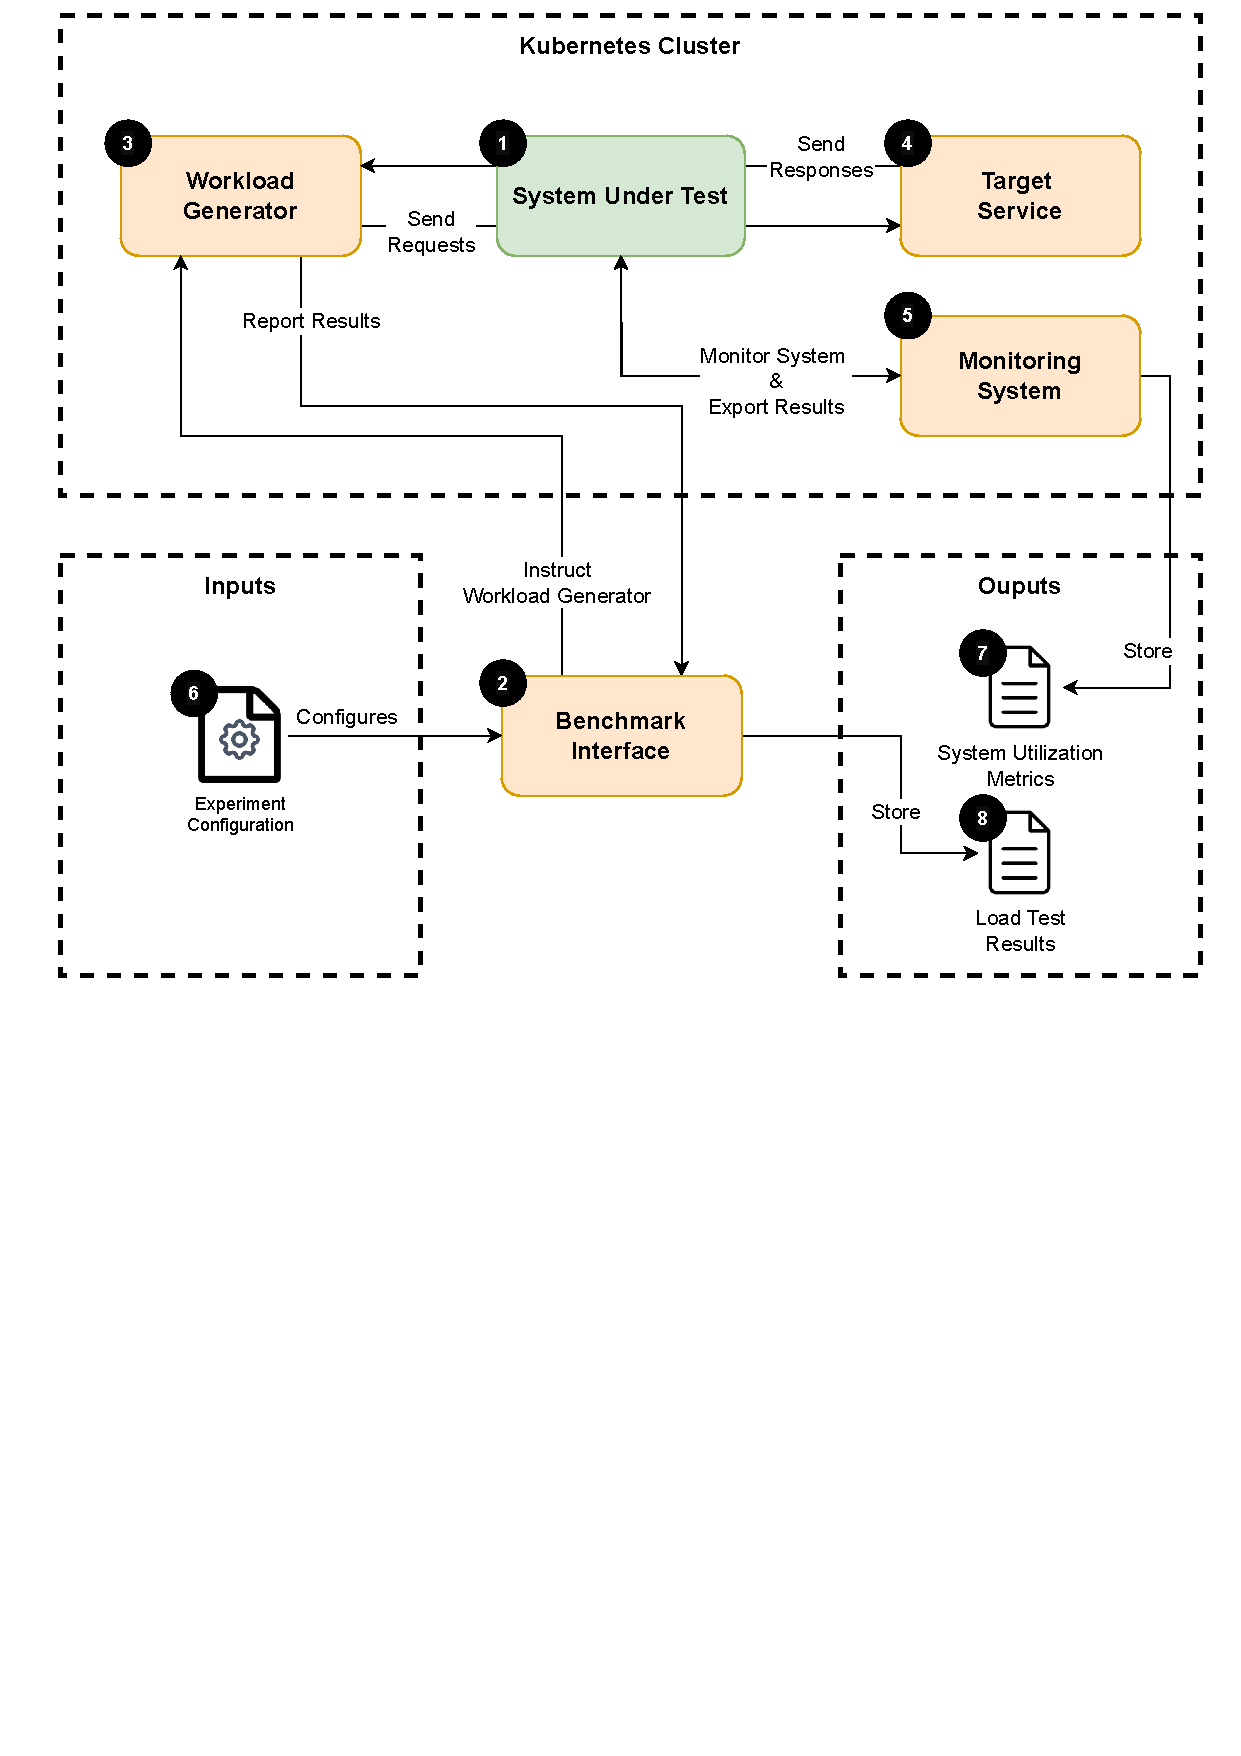
\includegraphics[width=0.9\linewidth]{4_system_design/figures/benchmark-design.pdf}
    
    \caption{\textit{MeshBench}, a benchmark for \gls{sm} systems.}
    
    \label{fig:benchmark-design}
\end{figure}



\subsection{System Under Test}
The \gls{sut} \designref{1} represents the heart of the benchmark. It contains the components of interest that we wish to evaluate and is explained in further detail in \label{sec:system:sut}. However, it is important to note that we introduced the notion of the \textit{application container} as a component of interest as part of the \gls{sut}. These application containers come in the form of the \textit{Workload Generator}\designref{3} and \textit{Target Service} \designref{4} as depicted in the design. We measure the network traffic between these application containers, which is expressed in the design by the arrows going beneath the \gls{sut}.

\subsection{Benchmark Interface}
The \textit{Benchmark Interface} \designref{2} is the entry point for the end user and enables them to perform performance experiments. The main goal of the Benchmark Interface is to manage experiment executions. The lifecycle of a single experiment consists of three phases. The first phase consists of initialization and configuration. This is done by parsing and processing an \textit{Experiment Configuration} \designref{6}. After this, it instructs the \textit{Workload Generator} \designref{3}, to generate experiment-specific workloads based on the supplied configuration. Once an experiment is finished and the workload generator has reported back to the benchmark interface, it finalizes the experiment and stores the obtained results.

\subsection{Workload Generator}
The \textit{Workload Generator} \designref{3} is used to generate synthetic workloads and measure the performance of the \gls{sut}. This is arguably the most important component in the benchmark, and it has to support various modes of operation to match the functional requirements as defined in \cref{sec:system:requirements-analysis:functional}. The workload generator has to be able to perform load test experiments, in which it generates a certain application workload for a \textit{Target Service} \designref{4}. It has to be able to do so in a constant throughput fashion, i.e. a fixed number of requests per second while also supporting a mode that enables us to test the maximum throughput of a given \gls{sut}. Another important aspect is that it should be configurable at run-time, so that the benchmark interface \designref{2} can configure it, allowing us to design various performance related experiments. 

The workload generator will be running inside the \textit{Kubernetes} cluster. More specifically, it will be part of the \gls{sut} itself. The workload generator will run as an application \gls{pod} in the cluster and will have a service proxy attached to it if the cluster is bootstrapped with a \gls{sm}. This ensures that the data path will traverse two application containers and two service proxies in meshed configurations.

\subsection{Target Service}
At the receiving end of the workload generator is a \textit{Target Service} \designref{4}. The goal of this component is to mimic a generic service as encountered in a production environment. However, the target service will take on a synthetic form and perform simple to no computations on the application workloads to minimize the impact on system resources and latencies observed in the experiments. An important note is that the target service component as depicted in the design can be multiple logical components, where each target is a synthetic service for a specific application workload e.g. HTTP, gRPC. This allows us to evaluate the performance characteristics of a \gls{sm} using different application level protocols.

\subsection{Monitoring System}
The \textit{Monitoring System} \designref{5} is responsible for monitoring the systems within the \textit{Kubernetes Cluster}. This is used primarily to collect system resource utilization metrics for all the components. The monitoring system has to support the collection of these metrics at a fine granularity. More specifically, it has to be able to distinguish resource utilization metrics at a pod and container granularity. This allows us to identify resource utilization patterns for the components of interest. The system should output these results in a common format to stable storage, or allow end users to query the data to export it in a common format \designref{7}.


\subsection{Experiment Configuration}
The benchmark consists of several performance experiments, as introduced in \cref{chap:experimental-evaluation}. Each of these experiments consists of several configuration parameters, which allows the user to change several aspects of the experiment. Notable configurations include the ability to modify the type of workload, the frequency of the workload, the duration of the experiment and the target service \designref{4}. These configuration parameters of a single experiment, forms the \textit{Experiment Configuration} \designref{6} and is the primary input of the benchmark interface \textbf{2}.

\subsection{System Utilization Metrics}
The \textit{System Utilization Metrics} \designref{7} contain experimental results regarding the system utilization metrics. More specifically, it contains time series data tied to an experiment regarding the CPU utilization and memory consumption. It is reported at the granularity of an application container which enables detailed analysis for components of the \gls{sut}.

\subsection{Load Test Results}
The \textit{Load Test Results} \designref{1} are the results created by the \textit{Workload Generator} \designref{3}. These results contain the performance results of an experiment. More specifically, it contains the request latencies as generated by the workload generator. Additionally, it comes with metadata  such as the experimental configuration and environment data. 
